% VerdeAI gap-analysis pipeline — research-paper figure.
%
% Standalone file: compiles on its own (e.g. on Overleaf) to a single
% cropped PDF/PNG you can \includegraphics{} directly.
%
% To embed inside an existing paper instead of using it standalone:
%   1. Copy everything from \begin{tikzpicture} to \end{tikzpicture}.
%   2. Paste it inside your own:
%        \begin{figure*}[t]
%          \centering
%          <paste tikzpicture here>
%          \caption{VerdeAI's document-to-gap-report pipeline. Shapes
%            follow standard flowchart convention: input/output,
%            decision, deterministic process, model-call
%            (``predefined process''), and document output.}
%          \label{fig:verdeai-pipeline}
%        \end{figure*}
%   3. Copy the \usetikzlibrary{...} line and the \definecolor / \tikzset
%      blocks into your own preamble (or a shared style file).
%
% The diagram is wide (7 columns). In a two-column paper, scale it to
% fit rather than shrinking font size, e.g.:
%   \resizebox{\linewidth}{!}{\includegraphics{verdeai-pipeline-figure}}
%
\documentclass[tikz, border=6mm]{standalone}
\usetikzlibrary{shapes.geometric, arrows.meta, positioning, calc}

% ---- palette: muted, print-safe. One hue per SHAPE CATEGORY (not per
% step), so the legend maps directly onto the shape vocabulary and the
% figure still reads correctly if printed in grayscale (shape carries
% the meaning; color is a redundant, secondary cue). ----
\definecolor{inkcolor}{HTML}{17241B}     % borders + text
\definecolor{mutedtext}{HTML}{4D5D4F}    % secondary/caption text
\definecolor{terminalfill}{HTML}{F2F3EF} % start / end
\definecolor{iofill}{HTML}{B7C6DA}       % input / output (parallelogram)
\definecolor{decisionfill}{HTML}{E6D3A3} % decision (diamond)
\definecolor{processfill}{HTML}{BFD3BC}  % deterministic process (rectangle)
\definecolor{aifill}{HTML}{CBB9D6}       % AI / model call (predefined process)
\definecolor{reportfill}{HTML}{3E5C43}   % final report (document shape)

\begin{document}
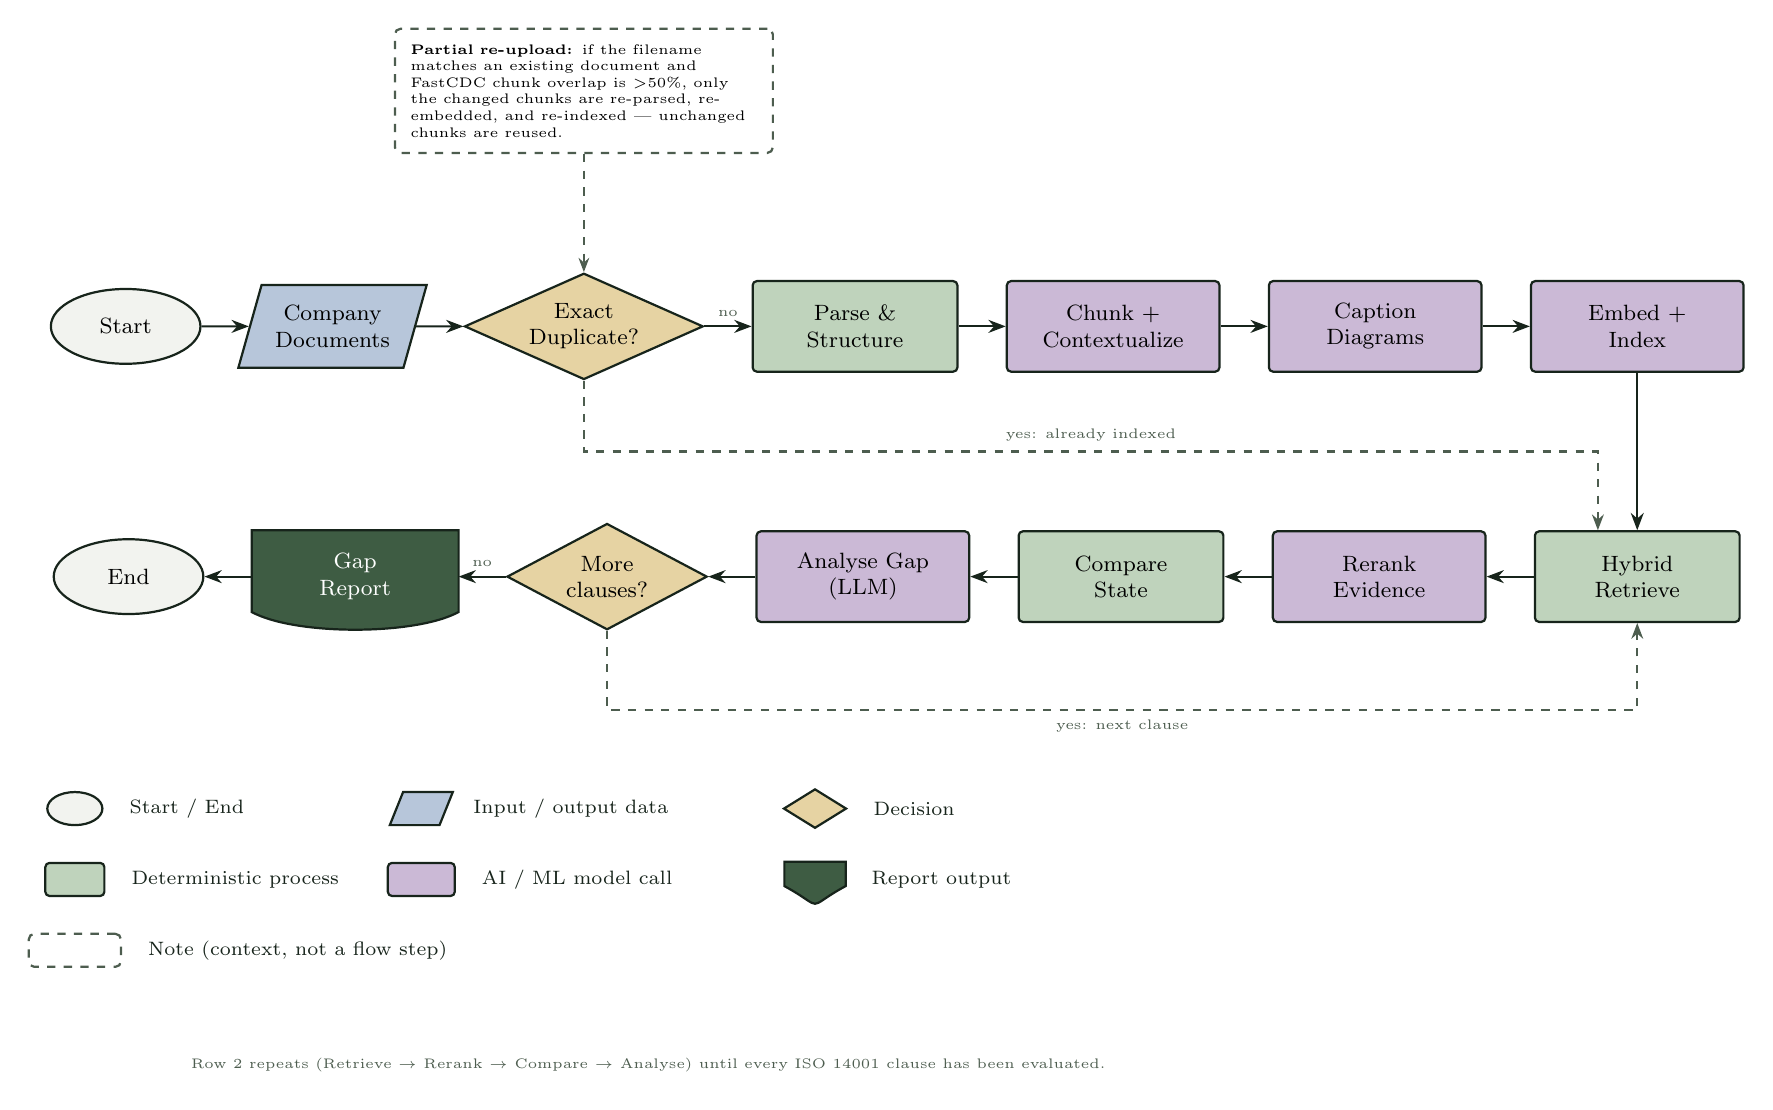
\begin{tikzpicture}[
  >=Stealth,
  every node/.style={font=\footnotesize},
  node distance=6mm and 6mm,
  align=center,
  thick,
]

% ---------------------------------------------------------------
% Node style vocabulary — one style per flowchart meaning.
% ---------------------------------------------------------------
\tikzset{
  terminal/.style={
    ellipse, draw=inkcolor, fill=terminalfill,
    minimum width=1.9cm, minimum height=0.95cm,
  },
  io/.style={
    trapezium, trapezium left angle=70, trapezium right angle=110,
    trapezium stretches=true,
    draw=inkcolor, fill=iofill,
    minimum width=2.4cm, minimum height=1.05cm,
  },
  decision/.style={
    diamond, draw=inkcolor, fill=decisionfill, aspect=2.4,
    inner sep=1pt, minimum width=2.5cm, minimum height=1.35cm,
  },
  process/.style={
    rectangle, rounded corners=1.5pt, draw=inkcolor, fill=processfill,
    minimum width=2.6cm, minimum height=1.15cm,
  },
  subprocess/.style={
    rectangle, rounded corners=1.5pt, draw=inkcolor, fill=aifill,
    minimum width=2.7cm, minimum height=1.15cm,
    append after command={
      \pgfextra{
        \draw[inkcolor]
          ($(\tikzlastnode.north west)!0.16cm!(\tikzlastnode.north east)$)
          -- ($(\tikzlastnode.south west)!0.16cm!(\tikzlastnode.south east)$);
        \draw[inkcolor]
          ($(\tikzlastnode.north east)!0.16cm!(\tikzlastnode.north west)$)
          -- ($(\tikzlastnode.south east)!0.16cm!(\tikzlastnode.south west)$);
      }
    },
  },
  flowline/.style={-{Stealth[length=2.2mm]}, inkcolor},
  branchline/.style={-{Stealth[length=2mm]}, mutedtext, dashed},
  annotation/.style={
    rectangle, rounded corners=2pt, draw=mutedtext, dashed, fill=white,
    text width=4.4cm, font=\tiny, align=left, inner sep=2mm,
  },
}

% Draws a hand-built "document" symbol (rectangle with a wavy bottom
% edge) at the position/size of an existing (invisible) node #1, with
% label text #2. Used instead of a named shape library so the file has
% no dependency beyond shapes.geometric.
\newcommand{\documentshape}[2]{
  \draw[inkcolor, fill=reportfill]
    (#1.north west) -- (#1.north east)
    -- ($(#1.south east)+(0,0.14)$)
    .. controls ($(#1.south east)+(-0.55,-0.16)$) and ($(#1.south west)+(0.55,-0.16)$) ..
    ($(#1.south west)+(0,0.14)$) -- cycle;
  \node[text=white, align=center] at (#1) {#2};
}

% =================================================================
% ROW 1 — document ingestion & indexing (left to right)
% =================================================================
\node[terminal]                              (start)    {Start};
\node[io,         right=of start]            (docs)     {Company\\Documents};
\node[decision,   right=of docs]             (dup)      {Exact\\Duplicate?};
\node[process,    right=of dup]              (parse)    {Parse \&\\Structure};
\node[subprocess, right=of parse]            (chunk)    {Chunk +\\Contextualize};
\node[subprocess, right=of chunk]            (caption)  {Caption\\Diagrams};
\node[subprocess, right=of caption]          (embed)    {Embed +\\Index};

% ---------------------------------------------------------------
% Annotation — the "no" path isn't only full/fresh processing: a
% re-upload that matches an existing filename but isn't byte-identical
% gets a scope optimisation, not a new branch (same boxes are visited,
% just less work inside them), so this is a note, not a diamond.
% ---------------------------------------------------------------
\node[annotation, above=15mm of dup] (note1)
  {\textbf{Partial re-upload:} if the filename matches an existing
  document and FastCDC chunk overlap is $>$50\%, only the changed
  chunks are re-parsed, re-embedded, and re-indexed --- unchanged
  chunks are reused.};
\draw[mutedtext, dashed, -{Stealth[length=1.8mm]}] (note1.south) -- (dup.north);

% =================================================================
% ROW 2 — per-clause gap analysis (right to left, below row 1)
% =================================================================
\node[process,    below=20mm of embed]       (retrieve) {Hybrid\\Retrieve};
\node[subprocess, left=of retrieve]          (rerank)   {Rerank\\Evidence};
\node[process,    left=of rerank]            (compare)  {Compare\\State};
\node[subprocess, left=of compare]           (analyse)  {Analyse Gap\\(LLM)};
\node[decision,   left=of analyse]           (more)     {More\\clauses?};
\node[rectangle, minimum width=2.6cm, minimum height=1.15cm,
      left=of more]                          (reportbox) {};
\node[terminal,   left=of reportbox]         (end)      {End};

% =================================================================
% Main flow — row 1
% =================================================================
\draw[flowline] (start) -- (docs);
\draw[flowline] (docs) -- (dup);
\draw[flowline] (dup) -- node[above, font=\tiny, text=mutedtext]{no} (parse);
\draw[flowline] (parse) -- (chunk);
\draw[flowline] (chunk) -- (caption);
\draw[flowline] (caption) -- (embed);

% bend: row 1 -> row 2
\draw[flowline] (embed.south) -- (retrieve.north);

% Main flow — row 2 (right to left)
\draw[flowline] (retrieve) -- (rerank);
\draw[flowline] (rerank) -- (compare);
\draw[flowline] (compare) -- (analyse);
\draw[flowline] (analyse) -- (more);
\draw[flowline] (more) -- node[above, font=\tiny, text=mutedtext]{no} (reportbox);
\draw[flowline] (reportbox) -- (end);

% =================================================================
% Branch 1 — duplicate short-circuit: skip straight to retrieval,
% the document's chunks are already indexed from a prior upload.
% Routed through the lane between row 1 and row 2, entering
% "Hybrid Retrieve" slightly left of center so it stays visually
% distinct from the main embed->retrieve arrow.
% =================================================================
\coordinate (bypassLane)  at ($(dup.south)+(0,-0.9)$);
\coordinate (bypassEntry) at ($(retrieve.north)+(-0.5,0)$);
\coordinate (bypassTurn)  at (bypassEntry |- bypassLane);
\draw[branchline]
  (dup.south) -- (bypassLane)
  -- node[above, font=\tiny, text=mutedtext]{yes: already indexed} (bypassTurn)
  -- (bypassEntry);

% =================================================================
% Branch 2 — loop back for the next ISO 14001 clause. Routed through
% a lane below row 2, re-entering "Hybrid Retrieve" from the south
% (unused by any other arrow).
% =================================================================
\coordinate (loopLane)  at ($(more.south)+(0,-1.0)$);
\coordinate (loopEntry) at (retrieve.south);
\coordinate (loopTurn)  at (loopEntry |- loopLane);
\draw[branchline]
  (more.south) -- (loopLane)
  -- node[below, font=\tiny, text=mutedtext]{yes: next clause} (loopTurn)
  -- (loopEntry);

% document (report) shape, drawn on top of its placeholder node
\documentshape{reportbox}{Gap\\Report}

% =================================================================
% Legend — placed below the whole diagram, clear of the loop-back lane.
% =================================================================
\begin{scope}[shift={($(end.south west)+(0,-2.6)$)}]
  \node[terminal, minimum width=0.7cm, minimum height=0.42cm, font=\tiny] (l1) at (0,0) {};
  \node[right=2mm of l1, font=\scriptsize, text=inkcolor] {Start / End};

  \node[io, minimum width=0.8cm, minimum height=0.42cm, font=\tiny] (l2) at (4.4,0) {};
  \node[right=2mm of l2, font=\scriptsize, text=inkcolor] {Input / output data};

  \node[decision, minimum width=0.8cm, minimum height=0.5cm, font=\tiny] (l3) at (9.4,0) {};
  \node[right=2mm of l3, font=\scriptsize, text=inkcolor] {Decision};

  \node[process, minimum width=0.75cm, minimum height=0.42cm, font=\tiny] (l4) at (0,-0.9) {};
  \node[right=2mm of l4, font=\scriptsize, text=inkcolor] {Deterministic process};

  \node[subprocess, minimum width=0.85cm, minimum height=0.42cm, font=\tiny] (l5) at (4.4,-0.9) {};
  \node[right=2mm of l5, font=\scriptsize, text=inkcolor] {AI / ML model call};

  \node[rectangle, minimum width=0.75cm, minimum height=0.42cm] (l6) at (9.4,-0.9) {};
  \documentshape{l6}{}
  \node[right=2mm of l6, font=\scriptsize, text=inkcolor] {Report output};

  \node[annotation, text width=1.1cm, minimum height=0.42cm, inner sep=1pt,
        font=\tiny] (l7) at (0,-1.8) {};
  \node[right=2mm of l7, font=\scriptsize, text=inkcolor] {Note (context, not a flow step)};
\end{scope}

\node[font=\tiny, text=mutedtext, below=6mm of end, xshift=6.6cm, yshift=-4.9cm]
  {Row 2 repeats (Retrieve $\rightarrow$ Rerank $\rightarrow$ Compare $\rightarrow$ Analyse) until every ISO 14001 clause has been evaluated.};

\end{tikzpicture}
\end{document}
